\section{Patterns 1 - GoF Strategy + GoF Template Method}

\subsection{Fokuspunkter}

\begin{itemize}
	\item Redegør for, hvad et Software Design Pattern er.
	\item Sammenlign de to design patterns GoF Strategy og GoF Template Method - hvornår vil du anvende hvilket, og hvorfor?
	\item Vis et designeksempel på anvendelsen af GoF Strategy.
	\item Redegør for, hvordan anvendelsen af GoF Templete fremmer godt SW design.
	\item Redegør for, hvilke(t) SOLID-princip(per) du mener anvendelsen af GoF Strategy understøtter.
\end{itemize}

\subsection{Hvad er et Software pattern?}

\derp

\subsection{Sammenlign de to design patterns GoF Strategy og GoF Template Method - hvornår vil du anvende hvilket, og hvorfor?}
De er begge herp derp noget gøgl.

\subsubsection{Forskelle og ligheder}

\subsubsection{GoF Strategy Pattern}
GoF strategy pattern er et Design Pattern, der gør det mulgt at ændre en algoritmes opførsel, runtime.

\paragraph{Et strategy pattern}
\begin{itemize}
	\item Definerer en \textit{familie} af algoritmer.
	\item Indkapsler hver algoritme. \todo{vil det sige i hver sin afledte klasse af interfacet??}
	\item Gør algoritmerne \textbf{\textit{interchangable}} i dennes familie.
\end{itemize}

På denne måde lader dette mønster disse algoritmer varierere alt efter hvad dets klienter ønsker.

\begin{figure}[h]
	\centering
	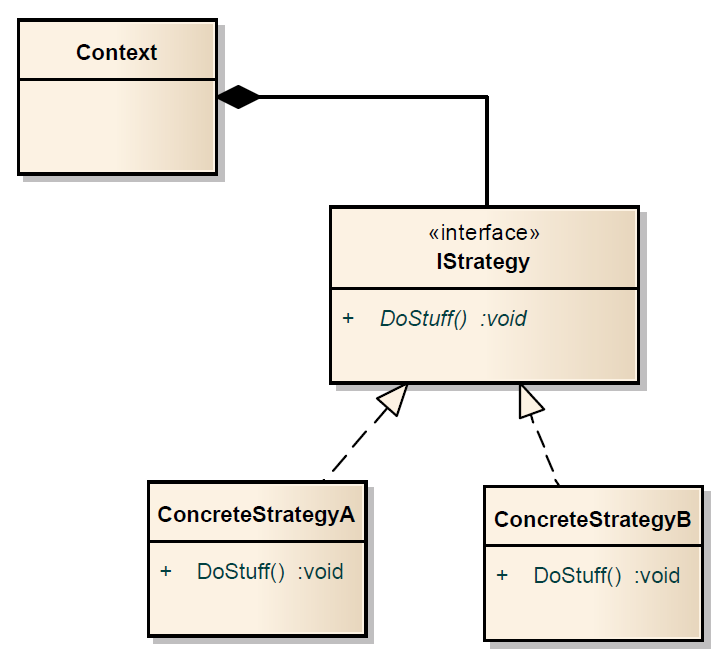
\includegraphics[width=0.6\linewidth]{figs/strategyPattern.PNG}
	\caption[UML for et strategy pattern]{Simpel illustration af et strategy pattern}
	\label{fig:strategyPattern}
\end{figure}

\subsection{Vis et designeksempel på anvendelsen af GoF Strategy}

Lad os tage udgangspunkt i figur~\ref{fig:strategyPattern}. Vores kontekst (klient) er en calculator der opererer på 2 integers.
Vi har da et ICalculator interface, med en enkelt virtuel metode, \textit{calculate()}.
Herudover har vi de 2 afledte klasser \textbf{Plus} og \textbf{Minus}.

Klientens constructor sætter det pågældende objekts strategy. Se main, hvor et client objekt oprettes og initialiseres.

\begin{lstlisting}
//Interface
 public interface ICalculate {
	 int Calculate(int value1, int value2);
 }

/*Concrete strategies*/

// Strategy 1: Minus
class Minus : ICalculate {
	public int Calculate(int value1, int value2) {
		return value1 - value2;
	}
}

//Strategy 2: Plus
class Plus : ICalculate {
	public int Calculate(int value1, int value2) {
		return value1 + value2;
	}
}

//klienten
class CalculateClient {
	private ICalculate calculateStrategy;

	//Constructor: assigns strategy to interface
	public CalculateClient(ICalculate strategy) {
		this.calculateStrategy = strategy;
	}

	//Executes the strategy
	public int Calculate(int value1, int value2) {
		return calculateStrategy.Calculate(value1, value2);
	}
}

//Initialisering
int application(object sender, EventArgs e) {
	CalculateClient minusClient = new CalculateClient(new Minus());
	Response.Write("<br />Minus: " + minusClient.Calculate(7, 1).ToString());

	CalculateClient plusClient = new CalculateClient(new Plus());
	Response.Write("<br />Plus: " + plusClient.Calculate(7, 1).ToString());
}

\end{lstlisting}

\subsection{Redegør for, hvilke(t) SOLID-princip(per) du mener anvendelsen af GoF Strategy understøtter}

\paragraph{Strategy Mønstret og OCP}
Som det kan ses på figur \ref{fig:strategyPattern}, er context (Klienten) open og closed, og OCP er herved overholdt. Klassen i sig selv bruger interfacet IStrategy, imens objekter af klienten bruger interfacets afledte klasser. Dette betyder, at hvis vi ønsker at bruge en ConcreteStrategyC skal vi ikke ændre noget i klient klassen. Vi skal derimod blot sætte klient objektet til at bruge den nye strategy.

\subsection{Redegør for, hvordan anvendelsen af GoF Templete fremmer godt SW design}
Hvis man har et system bestående af nogle klasser, hvor disse klasse funktionalitet kun afviger lidt fra hinanden. Så kan \textit{Template pattern} bruges. Via dette pattern kan et fast ''programflow'' defineres. Når dette ''flow'' så er fastlagt skal klasserne bare implementere/ændre (nok via override) de metoder som de ikke er tilfredse med.

\subsubsection{Eksempel på Template pattern}
Herunder er en abstrakt klasse der har metoder, som de mange spil bruger/følger. Eksemplet er taget fra \href{https://en.wikipedia.org/wiki/Template_method_pattern#Example_in_Java}{wikipedia} om template pattern

\begin{lstlisting}
abstract class Game {
	// Hook methods. Concrete implementation may differ in each subclass
	protected int PlayerCount;
	abstract void InitializeGame();
	abstract void MakePlay(int player);
	abstract void EndOfGame();
	abstract void AnnounceWinner();
	
	// A template method:
	public final void PlayGame(int playerCount)	{
		PlayerCount = playerCount;
		InitializeGame();
		int j = 0;
		while(!EndOfGame()) {
			MakePlay(j);
			j = (j + 1) % PlayerCount;
		}
		PrintWinner();
	}
}
\end{lstlisting}

Herunder ses så hvordan den specifikke implementering af den abstrakts klasse kan laves.

\begin{lstlisting}
class Monopoly : Game {
	/* Implementation of necessary concrete methods */
	void initializeGame() {
		// Initialize players
		// Initialize money
	}
	void makePlay(int player) {
		// Process one turn of player
	}
	boolean endOfGame() {
		// Return true if game is over 
		// according to Monopoly rules
	}
	void printWinner() {
		// Display who won
	}
	
	/* Specific declarations for the Monopoly game. */
	// ...
}
\end{lstlisting}





